\section{Base de données}
\label{sec:BD}


\subsection{Création de la base de données}
\label{subsec:creation-db}

La base de données est composée de trois tables contenant toutes les données utiles au bon fonctionnement du site.\\
Il y a la table \textbf{Users} \textit{pour tout ce qui concerne les utilisateurs}, la table \textbf{Results}, \textit{qui concerne les résultats de chaque chapitre} et la table \textbf{Tests} \textit{qui contient la liste des résultats}.

\begin{figure}[h]
  \centering
  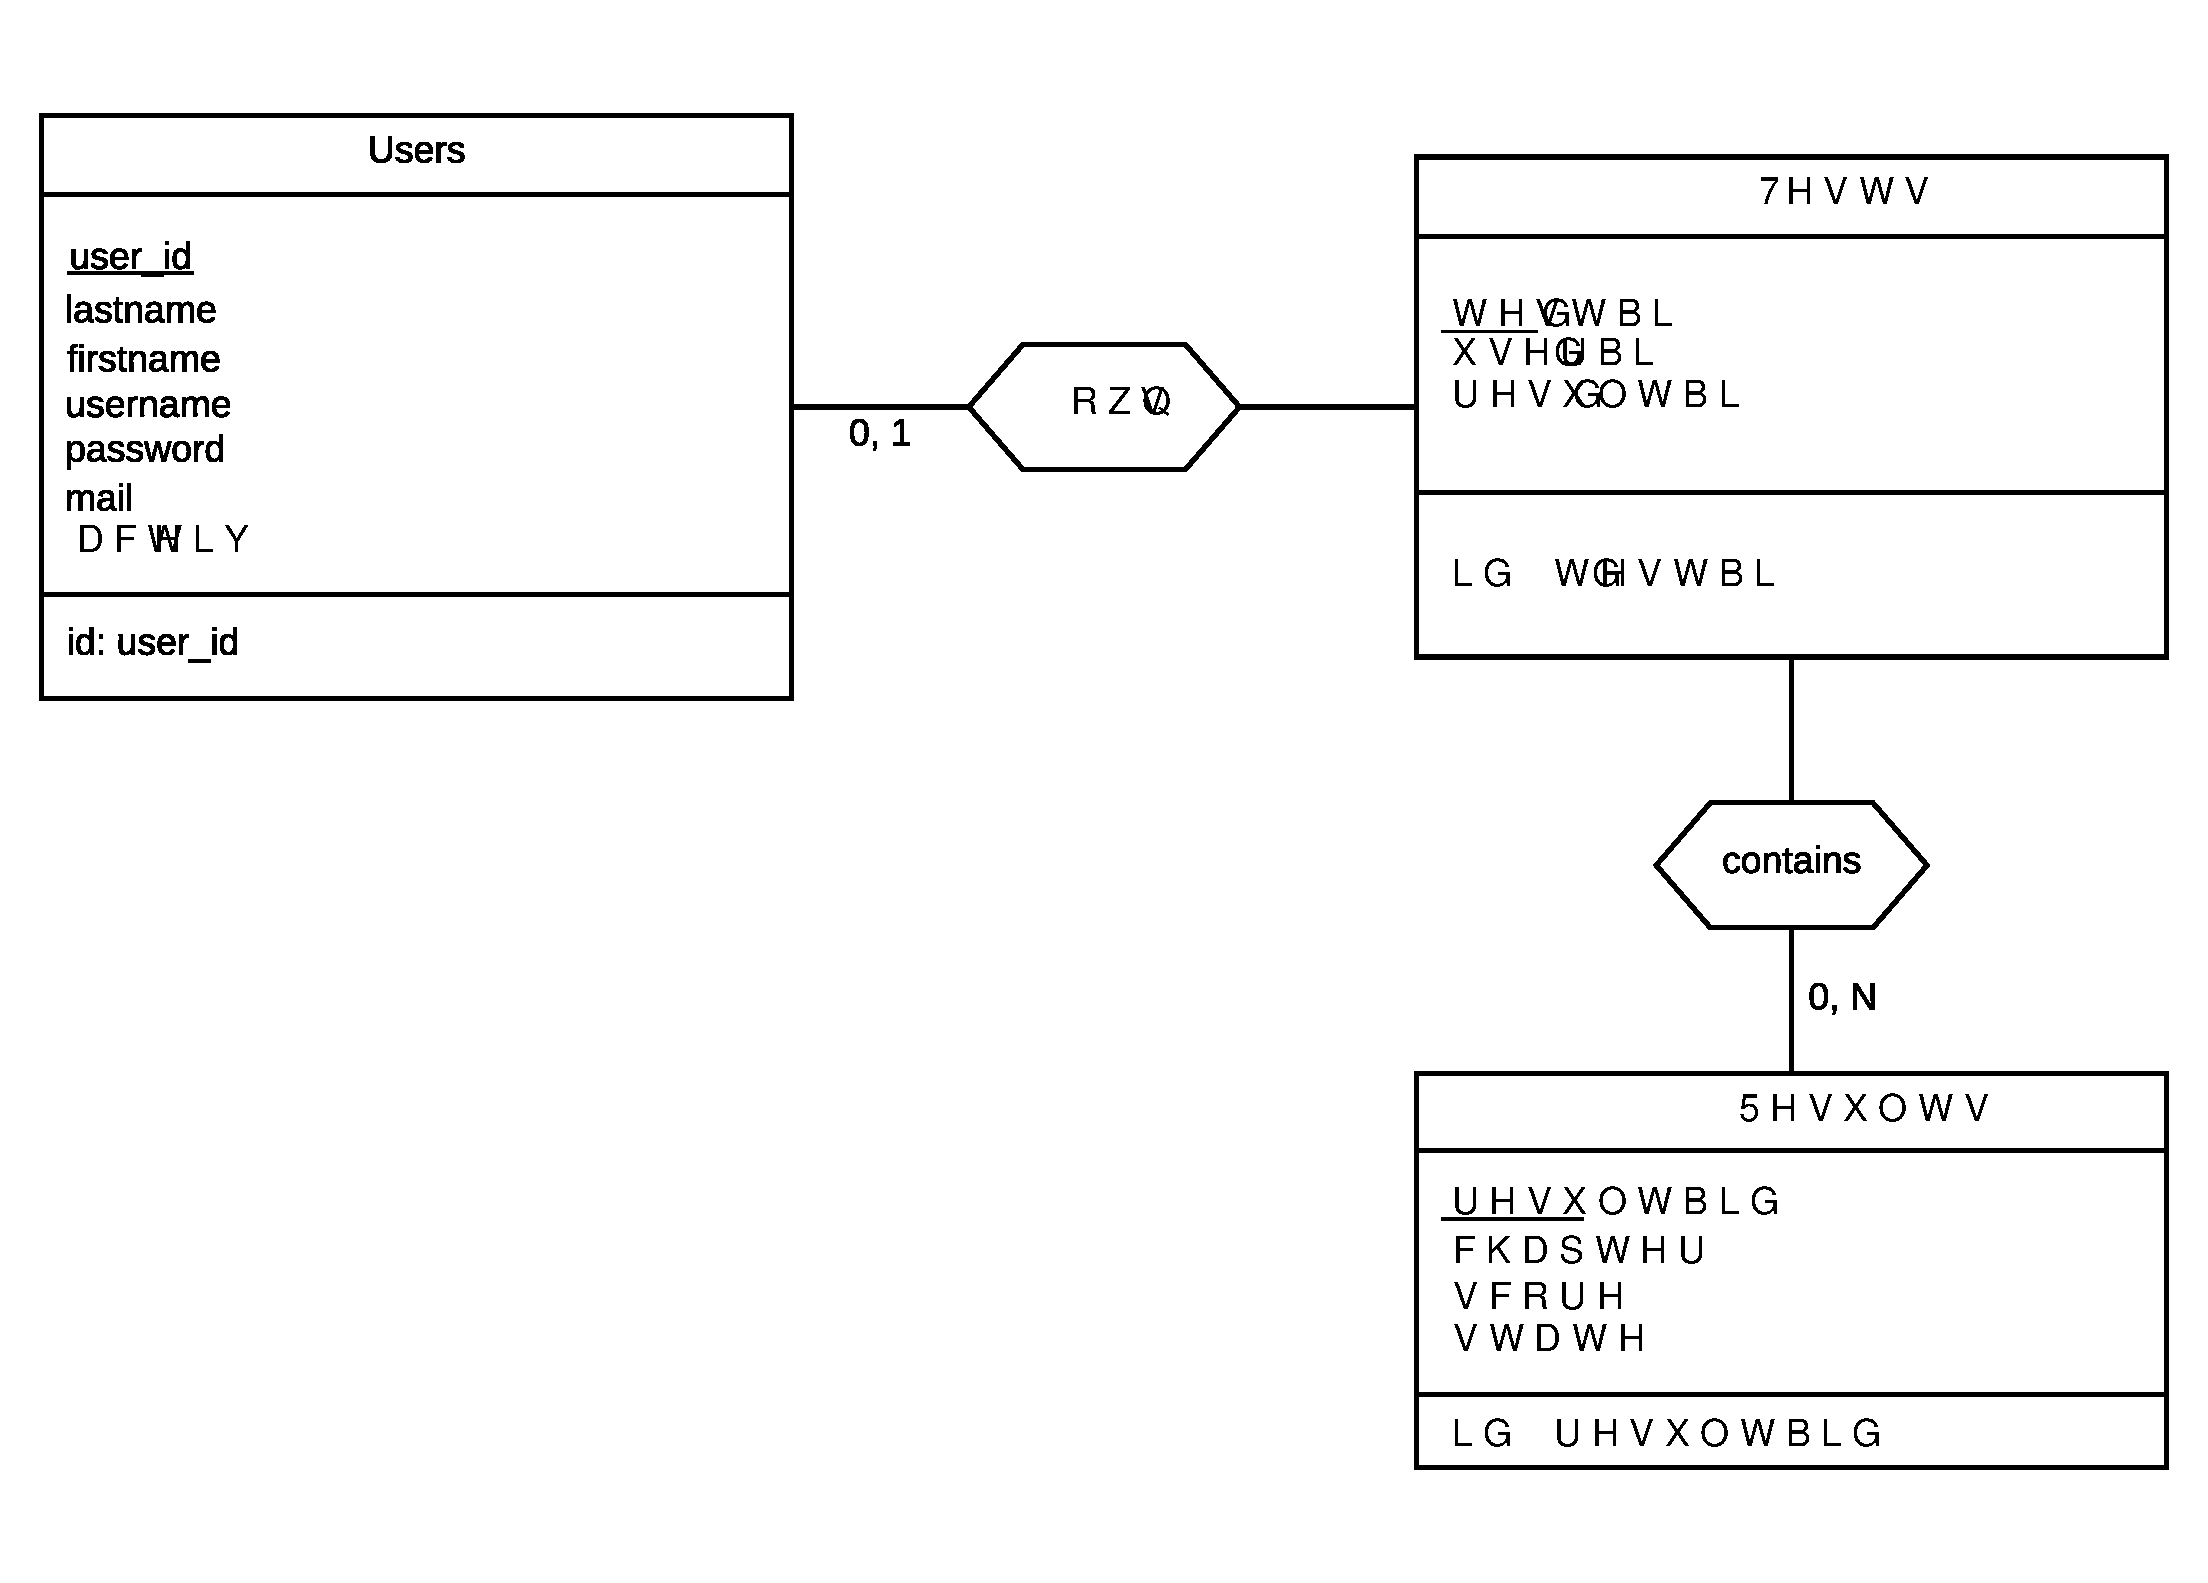
\includegraphics[scale=0.4]
  {textures/images/DB/DB.pdf}
  \caption{Schéma conceptuel de la base de données}
  \label{fig:db}
\end{figure}

\newpage


\subsection{Connexion à la base de données}
\label{subsec:conn-bd}

Le type de requêtes utilisé pour l'accès à la base de données est le type PDO.\\
De manière plus précise, ce sont des requêtes préparées qui ont été utilisées pour plus de sécurité \textit{(voir la section~\ref{subsec:securite}\textbf{~\nameref{subsec:securite}})}.\\
De plus, PDO permet plus de flexibilité. Elle est recommandée, très utilisée \textit{(et possède donc une importante communauté)} et est enseignée à l'école.\\

On pourrait alors ajouter, dans les évolutions possibles, le passage à la \textit{programmation orientée objet}, couplée à l’utilisation du \textit{singleton} et, comme structure de site, l’utilisation du \textit{design pattern \textbf{MVC}}.


\subsection{Sécurité}
\label{subsec:securite}

Pour la sécurité du site, tout accès à la base de données passe par des requêtes préparées \textit{(PDO)}, car celles-ci le protègent de toute injection SQL.\\

La connexion au site est surveillée grâce à la mise en place d’une session. Dès qu’un accès à une page se fait, la connexion est vérifiée. Si l’utilisateur n’est pas identifié, il est redirigé vers la page d’accueil.\\

En plus de cela, chaque champ de formulaire est protégé par des \textit{regex}\footnote{\href{https://fr.wikipedia.org/wiki/Expression\_rationnelle}{Expression régulière (en anglais: \textbf{Reg}ular \textbf{ex}pression)}}.\\
Celles-ci vérifient que les données entrées sont de la forme voulue: un nom ne doit contenir que des lettres et, selon une certaine forme, peut être divisé à l’aide d’un trait d’union; une adresse mail ne contient que des lettres minuscules non-accentuées, des points et un seul arobase; etc.\\

De plus, les mots de passe ont une longueur minimale de quatre caractères et doivent contenir, au moins, une majuscule, une minuscule et un chiffre.\\
Ils sont aussi \textit{hachés}\footnote{\url{https://fr.wikipedia.org/wiki/Fonction\_de\_hachage\_cryptographique}} à l’aide de \textit{SHA512} et d’un \textit{salage dynamique} pour plus de sécurité.\\
En effet, le mot de passe est de la forme \textbf{+\%\# longueur mot\_de\_passe  ¨*§}.\\ Par exemple, le mot de passe \textbf{Test1} devient \textbf{+\%\#5Test1¨*§} avant d’être haché.\\
Il est ainsi indéchiffrable, mais cela a aussi pour effet de sécuriser la base de données puisque le résultat ne contiendra que des caractères sûrs.



%%% Local Variables:
%%% mode: latex
%%% TeX-master: t
%%% End: